The existence of this data system is paramount to several automation tasks
in our lab. Below a few examples of the use of the data system for
these purposes are described.

\subsection{Morning pressure}\label{sec:morning_pressure}

As an example SQL statements can be used to plot the pressure in a vacuum
chamber at 1\,A.M. in the morning for the last month. This can be a useful tool
to monitor the general health of the chamber, i.e. if leaks has developed, a
valve is failing, a roughing pump is malfunctioning etc.

\begin{verbatim} 
select unix_timestamp(date(time)), avg(pressure) from
pressure_microreactor where hour(time) = 1 and minute(time) between 00 and 20
and time between {from} and {to} group by date(time) order by time desc limit
30; 
\end{verbatim}
where \{from\}  and \{to\} should be replaced with the
relevant time interval.

The output from as a statement like this is illustrated in
Figure~\ref{fig:morning_pressure}.
\begin{figure}
 \begin{center}
 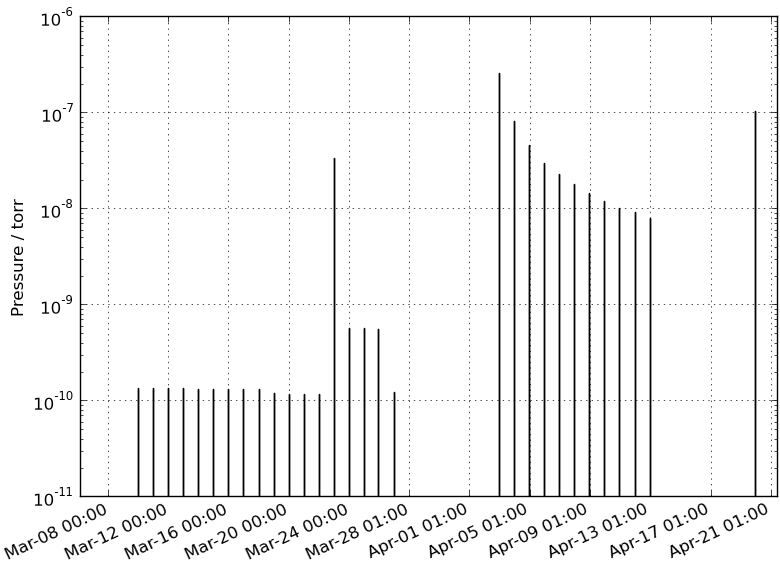
\includegraphics[width=10cm]{morning_pressure.png}
 \caption{ The morning pressure in a vacuum chamber at the department. The
   pressure gauge is unable to read high pressures, and thus no data is
   available from periods where the chamber is vented for maintenance.
   \label{fig:morning_pressure}
 } 
 \end{center}
\end{figure}

\subsection{Sample cleaning}
In the field of catalysis, one direction of research concerns gas
reactivity studies on the surface of single crystal samples under
Ultra High Vacuum (UHV)\fixme{Probably has been introduced before}
conditions ($\sim10^{-13}$\,mbar).

Before experiments can be performed, the sample must be properly
cleaned to ensure that no contaminants are present on the surface. The
cleaning of the surface is achieved by running a number of cleaning
cycles. Each of these cycles can take up to several hours.% and may
%include sputtering (bombardment of the surface with Ar$^+$ ions to
%peel or a part of the surface), gas exposure and heating.
Before this task was automatized, it typically required simple manual
intervention 2-4 times during a 30 to 120 minute cycle. Obviously, this
was a suboptimal solution, since a lot of time was spent, with only
small time intervals to work on other things, before the next manual
intervention.

As it is apparent that the atomization of this task lead to
significant time savings, since it allowed these cleaning cycles to
e.g.\ be run in the evening or at night. However, during the
atomization process one concerns that had to be addressed was how to
monitor the status of the cleaning and the equipment. With the data
logging system in place, all relevant parameters could easily be
continuously logged and viewed with any of the data viewing options
mentioned in section ???\fixme{insert ref}. Obviously the cleaning
program itself is responsible for the safety of the system and for
shutting it down if it goes out of boundaries. But with the continuous
logging it is a simple task to add surveillance to the cleaning that
alerts the user if it happens, which means that it can be safely
restarted if it is safe to do so. There is a specific case describing
a alarm in section \ref{sec:cooling_water_alarms}.

\subsection{Experimentation over extended time periods}

Mini-reactor example. Bla bla more exhaustive search of parameter
space for experiments with large time spans. \fixme{Finish section}

\subsection{Cooling water alarms}\label{sec:cooling_water_alarms}
*The access to a centralized point of storage for experimental data also allows
for real-time continuous logging of various parameters used as indicators for
system health. Critical system parameters can hence be monitored and used to
trigger alarms when these fall out of specified ranges. Furthermore, the
logging of experimental setup parameters continuously enables access to these
values at any previous point in time.

Several important pieces of equipment require cooling. If they loose
the cooling it will often result in equipment break down, which,
depending on the equipment, can be expensive both in repair cost and
work time lost.

In our lab the main components with critical cooling requirements are
the turbo molecular pumps that are used to maintain vacuum. We do not
have direct access to monitor the cooling water status. Therefore,
instead we mounted temperature measurements on all the pumps and log
all of the these via the data system. Then, on the server that runs
the data presentation website we added a script that fetches the
latest temperatures from the database, and if these start to climb,
sends out an alarm via email. While it was inconvenient that we were
unable to monitor the cooling water directly, this approach has the
very desirable side effect that we can now also monitor the health (to
the extent it is given by the temperature) of each pump
individually.\fixme{Decide if we want to mention this here or at all}
